\documentclass[24pt,pdf,hyperref={unicode},aspectratio=169]{beamer}
\usepackage[utf8]{inputenc}
\usepackage{aiml}
\begin{document}


\section{Введение в логику}



\begin{frame}\frametitle{Дедуктивные рассуждения}
\begin{tabular}{l l}
 & Все страны Южной Америки -- республики \\
 & Бразилия -- страна Южной Америки\\
 \hline
$\therefore$ & Бразилия -- республика \\
\end{tabular}
\end{frame}

\begin{frame}\frametitle{Дедуктивные рассуждения}
\begin{tabular}{l l}
 & Все страны Южной Америки -- республики \\
 & Китай -- это не страна Южной Америки\\
 \hline
$\therefore$ & Китай -- республика \\
\end{tabular}
\end{frame}

\begin{frame}\frametitle{Дедуктивные рассуждения}
\begin{tabular}{l l}
 & Все страны Азии -- республики \\
 & Тайланд -- это страна Азии\\
 \hline
$\therefore$ & Тайланд -- республика \\
\end{tabular}
\end{frame}

\begin{frame}\frametitle{Дедуктивные рассуждения}
\begin{tabular}{l l}
 & Все книги содержат буквы \\
 & <<Война и мир>> -- книга \\
 \hline
$\therefore$ & <<Война и мир>> содержит буквы\\
\end{tabular}
\end{frame}

\begin{frame}\frametitle{Дедуктивные рассуждения}
\begin{tabular}{l l}
 & Все $A$ есть $B$\\
 & Некоторый $x$ является $A$\\
 \hline
$\therefore$ & $x$ является $B$ \\
\end{tabular}
\end{frame}

\begin{frame}\frametitle{Дедуктивные рассуждения}
\begin{tabular}{l l}
 & У матери Джона есть дочь\\
 \hline
$\therefore$ & У Джона есть сестра \\
\end{tabular}
\end{frame}



\begin{frame}\frametitle{Индуктивные рассуждения}
\begin{tabular}{l l}
 & Бразилия -- страна Южной Америки и республика \\
 & Чили -- страна Южной Америки и республика \\
 & Уругвай -- страна Южной Америки и республика \\
\hline
$\therefore$ & Все страны Южной Америки -- республики \\
\end{tabular}
\end{frame}

\begin{frame}\frametitle{Индуктивные рассуждения}
\begin{tabular}{l l}
 & Франция -- страна Европы и республика \\
 & Германия -- страна Европы и республика \\
 & Чехия -- страна Европы и республика \\
\hline
$\therefore$ & Все страны Европы -- республики \\
\end{tabular}
\begin{flushright}
 \uncover<2>{
\includegraphics[width=4cm]{EnglishQueen.jpg}}
\end{flushright}
\end{frame}


\begin{frame}\frametitle{Индуктивные рассуждения}
\begin{tabular}{l l}
 & Бразилия -- республика и страна Южной Америки \\
 & Чили -- республика и страна Южной Америки \\
 & Уругвай -- республика и страна Южной Америки \\
\hline
$\therefore$ & Все республики -- страны Южной Америки\\
\end{tabular}
\begin{flushright}
 \uncover<2>{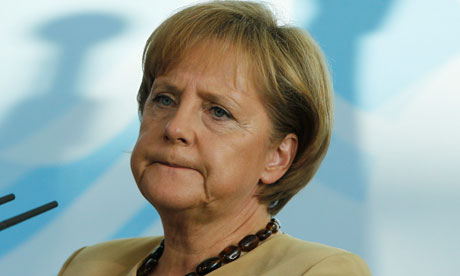
\includegraphics[width=4cm]{Merkel.jpg}}
\end{flushright}
\end{frame}


\end{document}
